\documentclass[conference]{IEEEtran}

\usepackage[spanish, bidi=basic, provide=*]{babel}
\babelprovide[import, onchar=ids fonts]{spanish}

\usepackage{subcaption}
\usepackage{graphicx}
\usepackage{amsmath}
\usepackage{tikz}
\usetikzlibrary{arrows.meta, positioning, fit, backgrounds}
\usepackage{float}
\usepackage[colorlinks=true, linkcolor=black, citecolor=black, urlcolor=blue]{hyperref}
\usepackage{dblfloatfix}
\usepackage{placeins}

\hyphenation{op-tical net-works semi-conduc-tor}

\begin{document}

\title{Clasificación Automática Multiclase de Estadios del Sueño mediante Inteligencia Artificial y Señales Polisomnográficas Multimodales}

\author{
\IEEEauthorblockN{
    Juan David Rozo Verástegui,
    Jhoan Sebastián Saavedra Romero\\
    Juan Javier Valera Mejías,
    Juan Carlos Gamboa Peñaranda
}
\IEEEauthorblockA{
    Maestría en Inteligencia Artificial\\
    Universidad de los Andes\\
    Bogotá, Colombia
}
}

\maketitle

\begin{abstract}
La polisomnografía (PSG) es el estándar de oro para diagnosticar trastornos del sueño, pero su estadificación manual constituye un cuello de botella operativo con alta variabilidad inter-evaluador en fases de transición. Este artículo presenta el diseño y evaluación de un ensamble híbrido desarrollado en cuatro fases de ablación (V4 a V7) sobre la base de datos pública \textit{Sleep-EDF Database Expanded}. La arquitectura final (V7) acopla una Red Neuronal Convolucional Recurrente (CRNN) de Fusión Tardía con contexto latente (192D) a partir de señales multimodales (EEG, EOG, EMG), junto a una rama espectral sub-época en bloques de 5 segundos (\textit{rFFT}) con normalización nocturna robusta ($P_{10}$--$P_{90}$) y contexto multiescala. El vector unificado de 528 dimensiones alimenta un clasificador LightGBM con aprendizaje sensible al costo y auditoría opcional mediante Modelos Ocultos de Markov (HMM). Evaluado sobre un conjunto de validación externa fijo de 20 noches estrictamente disjuntas por sujeto (10 sujetos de \textit{Sleep-Cassette}, 24,101 épocas), el perfil sin HMM (Exp 3) alcanzó 79.71\% de \textit{Accuracy}, 0.7286 en \textit{F1-Macro}, 0.7188 en Kappa y 0.41 en F1-N1. Al aplicar la auditoría HMM (Exp 4), el sistema obtuvo 79.93\% de \textit{Accuracy}, 0.7260 en \textit{F1-Macro}, 0.7211 en Kappa y 0.39 en F1-N1.
\end{abstract}

\begin{IEEEkeywords}
Clasificación de estadios del sueño, polisomnografía, redes neuronales convolucionales recurrentes, LightGBM, Modelos Ocultos de Markov, generalización multicohorte.
\end{IEEEkeywords}

\IEEEpeerreviewmaketitle

%===========================================================
\section{Introducción}
%===========================================================
El sueño es una función fisiológica esencial; su alteración crónica está directamente asociada con el desarrollo de patologías cardiovasculares, neurológicas, respiratorias y metabólicas. El estándar de oro para su diagnóstico clínico es la polisomnografía (PSG), que registra de forma continua bioseñales multimodales como la electroencefalografía (EEG), la electrooculografía (EOG) y la electromiografía (EMG). Un componente obligatorio de este análisis es la estadificación del sueño (\textit{sleep staging}), donde cada segmento de 30 segundos (época) se clasifica en uno de los cinco estadios definidos por la Academia Americana de Medicina del Sueño (AASM): Vigilia (W), N1, N2, N3 y REM \cite{berry2020}.

En la práctica clínica actual, la estadificación es estrictamente manual y exige revisar visualmente entre 800 y 1,200 épocas por paciente. Esto genera un cuello de botella operativo y financiero que retrasa la entrega de resultados. Además, las fases de transición como N1 presentan una elevada variabilidad inter-evaluador debido a su naturaleza breve y ambigua \cite{berry2020}, reflejando la complejidad de la microcontinuidad neuronal subyacente \cite{kemp2000}.

Desde la Inteligencia Artificial (IA), automatizar este proceso enfrenta dos retos principales: un severo desbalance clínico de clases y la heterogeneidad entre pacientes y equipos de registro (\textit{Domain Shift}). Aunque diversas arquitecturas alcanzan exactitudes prometedoras con canales aislados \cite{supratak2020}, suelen subutilizar la información multimodal y degradar su rendimiento fuera de su cohorte de origen.

En este trabajo se plantea la siguiente hipótesis: \textit{acoplar representaciones espaciotemporales profundas de una CRNN multimodal con descriptores espectrales sub-época (bloques de 5 s) normalizados por noche completa mejora el equilibrio multiclase y la detección de N1 frente a un esquema estrictamente local por época}. Para comprobarlo, se desarrolla un ensamble híbrido (CRNN + LightGBM \cite{ke2017} + HMM) concebido bajo principios MLOps como núcleo analítico del prototipo web \textit{SleepAI Studio}, orientado a asistir al especialista mediante un flujo futuro \textit{Human-in-the-Loop}.

%===========================================================
\section{Estado del Arte y Revisión Bibliográfica}
%===========================================================
El análisis automático de estadios del sueño ha evolucionado rápidamente. Los enfoques iniciales dependían de la extracción manual de características en tiempo y frecuencia acopladas a modelos clásicos como Máquinas de Vectores de Soporte (SVM) y Bosques Aleatorios, limitados por heurísticas rígidas.

Con el aprendizaje profundo (\textit{Deep Learning}), arquitecturas seminales como DeepSleepNet \cite{supratak2017} combinaron Redes Neuronales Convolucionales (CNN) unidimensionales con capas recurrentes (LSTM) directamente sobre señales crudas. Trabajos posteriores como U-Sleep \cite{perslev2021} y L-SeqSleepNet \cite{phan2023} escalaron el modelado a ciclos completos de sueño, mientras que propuestas como AttnSleep \cite{eldele2021} incorporaron mecanismos de atención para capturar dependencias temporales.

No obstante, un obstáculo persistente en el aprendizaje profundo es el desplazamiento de dominio (\textit{Domain Shift}). Como fenómeno general documentado en redes neuronales profundas, los modelos pueden recurrir a atajos predictivos (\textit{Shortcut Learning}) basados en correlaciones espurias del conjunto de entrenamiento en lugar de características generalizables \cite{geirhos2020shortcut}. En polisomnografía, esto se traduce en caídas de rendimiento al evaluar redes entrenadas en una única cohorte sobre poblaciones o equipos de registro distintos. Por ello, resulta fundamental emplear señales polisomnográficas directas (EEG, EOG y EMG) en lugar de aproximaciones periféricas como la fotopletismografía (PPG).

Desde la perspectiva neurofisiológica de la AASM \cite{berry2020}, cada estadio exhibe firmas espectrales distintivas: la Vigilia (W) presenta ritmo Alfa (8--12 Hz) y tono muscular elevado; N1 se define por la atenuación del ritmo Alfa en más del 50\% de la época y la aparición de ondas Theta (4--8 Hz) en microeventos de 10 a 15 segundos; N2 consolida husos de sueño (12--16 Hz) y complejos K; N3 muestra ondas lentas Delta (0.3--4 Hz) de alta amplitud; y REM combina actividad EEG mixta de bajo voltaje con movimientos oculares rápidos (EOG) y atonía muscular (EMG). Sin embargo, las CNN con promediado global (\textit{Global Average Pooling}) sobre 30 segundos tienden a diluir los microeventos breves de N1, y la normalización estrictamente local por época elimina la referencia de energía basal nocturna del paciente.

En este contexto, hibridar extractores profundos con motores tabulares enriquecidos espectralmente y post-procesamiento probabilístico mediante Modelos Ocultos de Markov (HMM) constituye una alternativa robusta para el modelado secuencial del sueño.

%===========================================================
\section{Metodología}
%===========================================================
La concepción metodológica se estructuró mediante un estudio de ablación progresivo. Cada iteración buscó resolver una limitación empírica de la fase anterior frente a la heterogeneidad biológica y técnica de los registros.

\subsection{Datos y Preprocesamiento de Señales}
El estudio se basó en la base de datos pública \textit{Sleep-EDF Database Expanded} \cite{sleepedfx_dataset}, \cite{goldberger2000}, fusionando dos cohortes:
\begin{itemize}
    \item \textbf{Cohorte Clínica (\textit{Sleep-Telemetry}):} 44 noches de 22 sujetos con trastornos del sueño leves.
    \item \textbf{Cohorte Externa (\textit{Sleep-Cassette}):} Las primeras 40 noches (21 sujetos únicos) se integraron al entrenamiento multicohorte. Para conformar el conjunto de validación externa fijo (\textit{Hold-Out}), se seleccionaron las siguientes 20 noches estrictamente disjuntas por sujeto (10 sujetos únicos, 24,101 épocas), excluyendo cualquier registro perteneciente a sujetos presentes en entrenamiento (0\% de fuga de sujeto).
\end{itemize}

El análisis exploratorio confirmó el desbalance estructural del sueño humano: N2 domina la distribución ($\approx$46.5\%), mientras que N1 representa una minoría crítica (8.6\%). Por ello se adoptó el \textit{F1-Score Macro} junto al Índice Kappa como métricas principales de evaluación.

Para evitar que la vigilia diurna prolongada de \textit{Sleep-Cassette} sesgue las métricas, todos los registros se recortaron conservando un margen estricto de $\pm$30 minutos antes del primer y después del último episodio de sueño (N1, N2, N3 o REM). El \textit{pipeline} base procesa cuatro canales (EEG Fpz-Cz, EEG Pz-Oz, EOG horizontal y EMG submental) mediante MNE-Python \cite{gramfort2013} (ver Figura \ref{fig:pipeline_stateless}). Dado que \textit{Sleep-Cassette} almacena la EMG submental como envolvente a baja frecuencia (1 Hz), la lectura con MNE remuestrea automáticamente todos los canales a 100 Hz (3,000 muestras por época). Se aplicó un filtro FIR pasabanda de fase cero (0.3--35.0 Hz) para preservar la morfología de los microeventos EEG \cite{berry2020}; se reconoce que este corte atenúa frecuencias altas de la EMG, limitando su rol a un indicador auxiliar de tono basal. Para garantizar continuidad operativa ante la ausencia física de canales auxiliares (siempre que exista al menos un canal EEG), el \textit{pipeline} implementa \textit{Zero Imputation} inyectando tensores nulos. Finalmente, la amplitud se estandarizó con Z-Score local por época para la rama profunda, complementada en V7 con normalización espectral nocturna.

\begin{figure}[htbp]
\centering
\resizebox{0.9\columnwidth}{!}{%
\begin{tikzpicture}[
    node distance=1.2cm and 1.5cm,
    box/.style={rectangle, draw=black, thick, fill=blue!5, text width=3.5cm, align=center, rounded corners, minimum height=1.2cm},
    arrow/.style={-{Stealth[scale=1.2]}, thick},
    group/.style={rectangle, draw=black, dashed, thick, inner sep=0.3cm, fill=gray!5}
]

\node[box, fill=green!10] (psg) {Lectura Dinámica\\(MNE-Python)};
\node[box, right=of psg] (filt) {Filtro FIR (Fase Cero)\\0.3 - 35.0 Hz};
\node[box, right=of filt] (norm) {Z-Score Local\\(Época a Época)};
\node[box, right=of norm] (tensor) {Imputación por Ceros\\(Tensores 3D)};

\draw[arrow] (psg) -- (filt);
\draw[arrow] (filt) -- (norm);
\draw[arrow] (norm) -- (tensor);

\begin{scope}[on background layer]
    \node[group, fit=(psg) (filt) (norm) (tensor), label={[font=\bfseries, text=black!70]above:Pipeline Base de Preprocesamiento \textit{Stateless}}] {};
\end{scope}

\end{tikzpicture}
}
\caption{Flujo de preprocesamiento analógico tolerante a fallos de sensores.}
\label{fig:pipeline_stateless}
\end{figure}

\subsection{Diseño Experimental y Entorno de Reproducibilidad}
Durante la fase exploratoria sobre la cohorte clínica (V4), se utilizó validación cruzada \textit{Leave-One-Subject-Out} (LOSO). Al escalar al entrenamiento multicohorte (V5 en adelante, 84 noches) con \textit{Data Augmentation} en memoria, LOSO resultó computacionalmente inviable y se transicionó a \textit{GroupKFold} de 5 pliegues agrupado por identificador único de sujeto (prefijos \texttt{ST\_} y \texttt{SC\_}).

Los entrenamientos se ejecutaron en Google Colab sobre GPU NVIDIA A100. La CRNN (246,053 parámetros) procesó secuencias de 15 épocas (\texttt{SEQ\_LEN=15}) con tamaño de lote de 128 (\texttt{BATCH\_SIZE=128}). La selección de hiperparámetros tabulares se realizó con Optuna (TPE) \cite{akiba2019optuna} y la calibración de pesos de clase en V7 empleó \textit{GroupShuffleSplit} (20\% validación interna, semilla 42).

\subsection{Evolución Arquitectónica (Estudio de Ablación)}
Previo a la arquitectura multimodal, tres prototipos exploratorios cualitativos guiaron el diseño: un \textit{Random Forest} sobre 1--2 canales EEG (V1), un motor tabular LightGBM básico (V2) y una CRNN con BiLSTM (V3) que no superó a V2, motivando la hibridación multimodal. A partir de ello se consolidó un ensamble de CRNN de Fusión Tardía \cite{supratak2017} (Figura \ref{fig:arq_v4}) acoplada a LightGBM \cite{ke2017}, refinado en cuatro fases (V4--V7):

% --- FIGURA COMPARATIVA V4 vs V7 ---
\begin{figure*}[htbp]
\centering

% --- MINIPAGE 1: MODELO V4 ---
\begin{minipage}{0.48\textwidth}
\centering
\resizebox{\linewidth}{!}{%
\begin{tikzpicture}[
    >=Latex,
    node distance=0.6cm and 0.5cm,
    font=\sffamily\small,
    input/.style={draw, rectangle, rounded corners, fill=blue!10, minimum width=2.5cm, minimum height=0.8cm, align=center},
    cnn/.style={draw, rectangle, fill=orange!15, minimum width=3cm, minimum height=1.5cm, align=center},
    fusion/.style={draw, rectangle, fill=gray!20, minimum width=5cm, minimum height=0.8cm, align=center},
    attention/.style={draw, ellipse, fill=yellow!20, minimum width=3cm, minimum height=0.8cm, align=center},
    lstm/.style={draw, rectangle, rounded corners, fill=green!15, minimum width=4cm, minimum height=0.8cm, align=center},
    dense/.style={draw, rectangle, fill=purple!15, minimum width=4cm, minimum height=0.8cm, align=center},
    lgbm/.style={draw, rectangle, dashed, thick, fill=blue!5, minimum width=4cm, minimum height=0.8cm, align=center},
    bgbox/.style={draw, rectangle, dashed, thick, inner sep=10pt, fill=black!2}
]

\node[input] (eog) {Entrada EOG \\ \scriptsize (15, 3000, 1)};
\node[input] (eeg) [left=0.5cm of eog] {Entrada EEG \\ \scriptsize (15, 3000, 2)};
\node[input] (emg) [right=0.5cm of eog] {Entrada EMG \\ \scriptsize (15, 3000, 1)};

\node[cnn] (cnneog) [below=of eog] {Conv1D (32) + BN \\ MaxPool1D (8) \\ GlobalAvgPool};
\node[cnn] (cnneeg) [below=of eeg] {Conv1D (64) + BN \\ MaxPool (8) \\ Conv1D (128) + BN \\ MaxPool (4) \\ GlobalAvgPool};
\node[cnn] (cnnemg) [below=of emg] {Conv1D (32) + BN \\ MaxPool1D (8) \\ GlobalAvgPool};

\begin{scope}[on background layer]
    \node[bgbox, fit=(eeg)(emg)(cnneeg)(cnnemg), label={[anchor=south west]north west:\textbf{Capa TimeDistributed (Secuencia T=15)}}] (tdbox) {};
\end{scope}

\node[fusion] (concat) [below=0.8cm of cnneog] {Concatenación Espacial};
\node[attention] (att) [below=0.5cm of concat] {Atención Espacial};
\node[lstm] (bilstm) [below=0.5cm of att] {BiLSTM (64 Unidades)};
\node[dense] (embeddings) [below=0.5cm of bilstm] {Capa Densa (64D)};
\node[lgbm] (lgbm_node) [below=0.5cm of embeddings] {Clasificador LightGBM \\ \scriptsize (Parámetros Manuales)};

\draw[->, thick] (eeg) -- (cnneeg);
\draw[->, thick] (eog) -- (cnneog);
\draw[->, thick] (emg) -- (cnnemg);
\draw[->, thick] (cnneeg.south) -- ++(0,-0.3) -| (concat.160);
\draw[->, thick] (cnneog.south) -- (concat.north);
\draw[->, thick] (cnnemg.south) -- ++(0,-0.3) -| (concat.20);
\draw[->, thick] (concat) -- (att);
\draw[->, thick] (att) -- (bilstm);
\draw[->, thick] (bilstm) -- (embeddings);
\draw[->, thick] (embeddings) -- (lgbm_node);
\end{tikzpicture}%
}
\caption{Fase I: Arquitectura Ensamble V4 (Línea Base Clínica).}
\label{fig:arq_v4}
\end{minipage}
\hfill
% --- MINIPAGE 2: MODELO V7 ---
\begin{minipage}{0.48\textwidth}
\centering
\resizebox{\linewidth}{!}{%
\begin{tikzpicture}[
    >=Latex,
    node distance=0.5cm and 0.4cm,
    font=\sffamily\small,
    input/.style={draw, rectangle, rounded corners, fill=blue!10, minimum width=2.4cm, minimum height=0.8cm, align=center},
    cnn/.style={draw, rectangle, fill=orange!15, minimum width=2.8cm, minimum height=1.3cm, align=center},
    spec/.style={draw, rectangle, rounded corners, fill=cyan!12, minimum width=3.2cm, minimum height=1.1cm, align=center},
    fusion/.style={draw, rectangle, fill=gray!20, minimum width=4.6cm, minimum height=0.7cm, align=center},
    attention/.style={draw, ellipse, fill=yellow!20, minimum width=2.8cm, minimum height=0.7cm, align=center},
    lstm/.style={draw, rectangle, rounded corners, fill=green!15, minimum width=3.8cm, minimum height=0.7cm, align=center},
    dense/.style={draw, rectangle, fill=purple!15, minimum width=3.8cm, minimum height=0.7cm, align=center},
    context/.style={draw, rectangle, rounded corners, fill=teal!15, minimum width=3.8cm, minimum height=0.75cm, align=center},
    lgbm/.style={draw, rectangle, thick, fill=blue!20, minimum width=4.8cm, minimum height=0.8cm, align=center},
    hmm/.style={draw, rectangle, dashed, rounded corners, fill=red!12, minimum width=4.8cm, minimum height=0.75cm, align=center},
    bgbox/.style={draw, rectangle, dashed, thick, inner sep=8pt, fill=black!2}
]

\node[input] (eog) {EOG + Noise/Drop \\ \scriptsize (15, 3000, 1)};
\node[input] (eeg) [left=0.35cm of eog] {EEG + Noise/Drop \\ \scriptsize (15, 3000, 2)};
\node[input] (emg) [right=0.35cm of eog] {EMG + Noise/Drop \\ \scriptsize (15, 3000, 1)};

\node[cnn] (cnneog) [below=of eog] {Conv1D (32) + BN \\ MaxPool1D (8) \\ GlobalAvgPool};
\node[cnn] (cnneeg) [below=of eeg] {Conv1D (64) + BN \\ Conv1D (128) + BN \\ GlobalAvgPool};
\node[cnn] (cnnemg) [below=of emg] {Conv1D (32) + BN \\ MaxPool1D (8) \\ GlobalAvgPool};

\begin{scope}[on background layer]
    \node[bgbox, fit=(eeg)(emg)(cnneeg)(cnnemg), label={[anchor=south west]north west:\textbf{Rama Profunda TimeDistributed (T=15)}}] (tdbox) {};
\end{scope}

\node[fusion] (concat) [below=0.6cm of cnneog] {Concatenación + Atención Espacial};
\node[lstm] (bilstm) [below=0.4cm of concat] {BiLSTM (64) + Densa (64D)};
\node[context] (context192) [below=0.4cm of bilstm] {Contexto CRNN (192D) \\ \scriptsize $E_{t-1} \oplus E_{t} \oplus E_{t+1}$};

\node[spec] (spec_branch) [right=0.5cm of context192] {Rama Espectral 5s (rFFT) \\ \scriptsize + Norm. Nocturna (P10--P90) \\ \scriptsize + Contexto 2m/7.5m (336D)};

\node[lgbm] (lgbm_node) [below=0.8cm of context192, xshift=1.8cm] {LightGBM Universal (528D) \\ \scriptsize Optuna + Pesos \texttt{Agresivo\_N1}};
\node[hmm] (hmm_node) [below=0.45cm of lgbm_node] {Auditoría Biológica HMM (Viterbi) \\ \scriptsize (Opcional: Máx. Acc/Kappa vs. F1-N1)};

\draw[->, thick] (eeg) -- (cnneeg);
\draw[->, thick] (eog) -- (cnneog);
\draw[->, thick] (emg) -- (cnnemg);
\draw[->, thick] (cnneeg.south) -- ++(0,-0.25) -| (concat.160);
\draw[->, thick] (cnneog.south) -- (concat.north);
\draw[->, thick] (cnnemg.south) -- ++(0,-0.25) -| (concat.20);
\draw[->, thick] (concat) -- (bilstm);
\draw[->, thick] (bilstm) -- (context192);
\draw[->, thick] (context192.south) -- ++(0,-0.3) -| (lgbm_node.150);
\draw[->, thick] (spec_branch.south) -- ++(0,-0.3) -| (lgbm_node.30);
\draw[->, thick] (lgbm_node) -- (hmm_node);
\end{tikzpicture}%
}
\caption{Fase IV: Arquitectura Ensamble Final (V7 --- 528D) con fusión espectral sub-época, normalización nocturna y calibración de costos.}
\label{fig:arq_v7}
\end{minipage}

\end{figure*}

\subsubsection{Fase I - Línea Base Clínica y Ensamble Tabular (V4)}
Se entrenó la CRNN multirrama exclusivamente sobre \textit{Telemetry} y se evaluó sobre las 20 noches limpias de \textit{Cassette} para cuantificar la caída de rendimiento entre cohortes. Posteriormente, la CRNN se truncó en su penúltima capa como extractor de 64 dimensiones (64D) para alimentar un clasificador LightGBM \cite{ke2017} con parámetros manuales, primero sobre \textit{Telemetry} y luego incorporando \textit{Cassette}.

\subsubsection{Fase II - Entrenamiento Multicohorte y Optimización (V5)}
Se integraron las 40 noches de \textit{Cassette} al entrenamiento de la CRNN para habilitar la generalización multicohorte. Con el fin de regularizar el espacio latente frente a posibles correlaciones espurias (\textit{Shortcut Learning}) \cite{geirhos2020shortcut}, se aplicó \textit{Data Augmentation} en GPU (\textit{Gaussian Noise} $\sigma=0.15$ y \textit{Spatial Dropout} 0.20). Se evaluaron dos configuraciones: ``V5 Base'' (parámetros tabulares heredados de V4) y ``V5 Óptima'', que integró optimización bayesiana con Optuna \cite{akiba2019optuna} y ajustó el factor $\gamma$ de la \textit{Categorical Focal Loss} \cite{lin2017} de 2.0 a 1.5 (Cuadro \ref{tab:hiperparametros}):
\begin{equation}
\mathcal{L}_{\text{FL}}(\mathbf{y}, \hat{\mathbf{p}}) = -\sum_{c=1}^{5} y_c (1 - \hat{p}_c)^{\gamma} \log(\hat{p}_c)
\label{eq:focal_loss}
\end{equation}

\begin{table}[htbp]
\centering
\caption{Resumen de Cambios en el Entrenamiento de la CRNN (246,053 Parámetros, LR=0.000125, Latente=64D, Dropout Max=0.4)}
\label{tab:hiperparametros}
\resizebox{\columnwidth}{!}{%
\begin{tabular}{|l|c|c|c|}
\hline
\textbf{Parámetro / Técnica} & \textbf{V4} & \textbf{V5 Base} & \textbf{V5 Óptima} \\ \hline
Cohorte de Entrenamiento & Telemetry & Tel. + Cas. & Tel. + Cas. \\ \hline
Focal Loss ($\gamma$) & 2.0 & 2.0 & 1.5 \\ \hline
Data Augmentation (Noise/Drop) & No & 0.15 / 0.20 & 0.15 / 0.20 \\ \hline
Optimización LightGBM & Manual & Manual & Optuna (TPE) \\ \hline
\end{tabular}%
}
\end{table}

\subsubsection{Fase III - Expansión Contextual y Auditoría HMM (V6)}
Utilizando el extractor CRNN de V5 Óptima, se concatenaron los vectores latentes de la época actual y sus vecinas ($E_{t-1} \oplus E_t \oplus E_{t+1}$), triplicando la entrada tabular a 192D. Para controlar el sobreajuste, Optuna elevó la regularización $L_1$ y $L_2$ (Cuadro \ref{tab:hiperparametros_reducida}). Finalmente, las probabilidades de emisión se auditaron mediante un Modelo Oculto de Markov (HMM) con decodificación de Viterbi en espacio logarítmico:
\begin{equation}
\delta_t(j) = \max_{i \in \mathcal{S}} \left[\delta_{t-1}(i) + \log A_{i,j}\right] + \log P(y_t = j \mid \mathbf{x}_t)
\label{eq:viterbi}
\end{equation}
donde $\mathcal{S} = \{\text{W, N1, N2, N3, REM}\}$ y $A_{i,j}$ es la matriz de transición estimada sobre las 84 noches de entrenamiento. En V6 se evaluaron cuatro etapas: Fase A (CRNN directa), Fase B (Ensamble 192D), Fase C (+ HMM) y Fase D (+ \textit{Test-Time Augmentation} de 5 pasadas + HMM).

\begin{table}[htbp]
\centering
\caption{Evolución de Hiperparámetros del Ensamble LightGBM}
\label{tab:hiperparametros_reducida}
\resizebox{\columnwidth}{!}{%
\begin{tabular}{lccc}
\hline
\textbf{Hiperparámetro} & \textbf{V4 (Baseline)} & \textbf{V5 Óptima} & \textbf{V6 / V7 (Base)} \\ \hline
\textbf{Contexto Latente (Dim)} & 64 & 64 & 192 (V7: 528) \\
\textbf{n\_estimators} & 300 & 500 & 600 \\
\textbf{learning\_rate} & 0.0500 & 0.0771 & 0.0644 \\
\textbf{max\_depth} & -1 & 7 & 7 \\
\textbf{num\_leaves} & 31 & 55 & 62 \\
\textbf{min\_child\_samples} & 20 & 120 & 130 \\
\textbf{subsample} & 1.0000 & 0.9137 & 0.7436 \\
\textbf{colsample\_bytree} & 1.0000 & 0.5539 & 0.5836 \\
\textbf{reg\_alpha (L1)} & 0.0000 & 0.0216 & 0.3760 \\
\textbf{reg\_lambda (L2)} & 0.0000 & 0.4921 & 1.4647 \\ \hline
\end{tabular}%
}
\end{table}

\subsubsection{Fase IV - Fusión Espectral Sub-Época y Calibración de Costos (V7 Final)}
El análisis de errores de V6 sugirió dos limitaciones en N1: el promediado global de 30 s en la CRNN diluye microeventos breves, y el Z-Score local elimina la referencia espectral nocturna. Manteniendo congelados el extractor CRNN (192D) y los hiperparámetros base de LightGBM (Cuadro \ref{tab:hiperparametros_reducida}), se ejecutaron cuatro experimentos incrementales (Figura \ref{fig:arq_v7}):
\begin{itemize}
    \item \textbf{Experimento 1 (Bloques Espectrales de 5 s --- 336D):} Cada época de 30 s se dividió en 6 bloques de 5 s ($N_b = 500$). Mediante \textit{rFFT} con ventana de Hann ($w_{\text{Hann}}$), se calculó la potencia logarítmica en 6 bandas clínicas $F_k$ (0.3--4, 4--8, 8--12, 12--16, 16--30 y 30--35 Hz) para los 4 canales:
    \begin{multline}
    S_{b,k,c} = \log\!\Bigg(1 + \frac{1}{|F_k|} \\
    \sum_{f \in F_k} \frac{\left|\text{rFFT}(x_{b,c} \cdot w_{\text{Hann}})_f\right|^2}{N_b}\Bigg)
    \label{eq:rfft_power}
    \end{multline}
    sumando $6 \times 6 \times 4 = 144$ características al vector de 192D.
    \item \textbf{Experimento 2 (Normalización Nocturna y Contexto Multiescala --- 528D):} Sobre las $m \in \{1,\dots,24\}$ combinaciones banda-canal se aplicó normalización robusta por registro nocturno usando mediana ($P_{50,m}$) y rango interdecil ($P_{90,m} - P_{10,m}$):
    \begin{equation}
    z_{t,b,m} = \operatorname{clip}\!\left(\frac{S_{t,b,m} - P_{50,m}}{\max(P_{90,m} - P_{10,m},\, 0.05)},\, -5,\, 5\right)
    \label{eq:robust_norm}
    \end{equation}
    aportando 144 descriptores. Sobre el promedio intra-época $\bar{z}_{t,m}$ se añadieron dos ventanas de contexto (media de 2 min y convolución triangular centrada de 7.5 min, +48 descriptores), totalizando 528D.
    \item \textbf{Experimento 3 (Aprendizaje Sensible al Costo):} Mediante validación interna (\textit{GroupShuffleSplit}, 20\%, semilla 42) se evaluaron tres perfiles de pesos por clase: \texttt{Moderado\_N1}, \texttt{Ref\_DART} y \texttt{Agresivo\_N1}. El perfil seleccionado (\texttt{Agresivo\_N1}: W=1.5, N1=3.5, N2=0.5, N3=1.3, REM=1.0) priorizó la sensibilidad en N1 moderando la dominancia de N2.
    \item \textbf{Experimento 4 (Auditoría HMM sobre V7):} Se aplicó Viterbi (Ec. \eqref{eq:viterbi}) noche por noche sobre las probabilidades del Exp 3, omitiendo el TTA de V6 para aislar el aporte determinista de 528D + HMM.
\end{itemize}

%===========================================================
\section{Resultados}
%===========================================================

La evaluación se enfocó en el conjunto de validación externa fijo (\textit{Hold-Out} limpio: 20 noches de 10 sujetos estrictamente disjuntos de \textit{Sleep-Cassette}, 24,101 épocas) para medir el comportamiento del sistema a lo largo de la ablación V4--V7.

\subsection{Caída de Rendimiento entre Cohortes (V4)}
La CRNN fundacional (V4), entrenada únicamente sobre \textit{Telemetry}, alcanzó un \textit{Accuracy} de 81.84\% y un Índice Kappa de 0.7396 en una validación interna preliminar Mini-LOSO (5 sujetos). Al evaluarse sobre las 20 noches externas de \textit{Cassette} (Cuadro \ref{tab:global_metrics}), el rendimiento descendió a 67.24\% de \textit{Accuracy} y 0.5728 de Kappa. Aunque ambos protocolos no son estrictamente equivalentes en tamaño muestral, la magnitud de la caída evidencia una fuerte sensibilidad al \textit{Domain Shift}. Como hipótesis plausibles de este comportamiento se plantean tanto diferencias poblacionales y de protocolo entre cohortes (sujetos con trastornos leves frente a normotípicos) como un posible fenómeno de \textit{Shortcut Learning} \cite{geirhos2020shortcut} sobre artefactos propios del equipo de registro.

\subsection{Rendimiento Global e Impacto Arquitectónico}
El Cuadro \ref{tab:global_metrics} resume la evolución de las métricas sobre el conjunto de validación externa fijo sin fuga de sujetos.

\begin{table}[htbp]
\centering
\caption{Evolución del Rendimiento Global en Validación Externa Limpia (20 Noches, 10 Sujetos Disjuntos, 24,101 Épocas)}
\label{tab:global_metrics}
\resizebox{\columnwidth}{!}{%
\begin{tabular}{|l|c|c|c|}
\hline
\textbf{Modelo / Fase de Ablación} & \textbf{Accuracy} & \textbf{F1-Macro} & \textbf{Kappa} \\ \hline
V4 (CRNN Pura - \textit{Baseline}) & 0.6724 & 0.6158 & 0.5728 \\ \hline
V4 (Ensamble LightGBM Simple) & 0.6961 & 0.6401 & 0.5969 \\ \hline
V4 (LGBM Telemetry+Cassette) & 0.7582 & 0.6822 & 0.6690 \\ \hline
V5 Base (CRNN + \textit{Data Augmentation}) & 0.7486 & 0.6833 & 0.6587 \\ \hline
V5 Base (LightGBM) & 0.7737 & 0.7093 & 0.6869 \\ \hline
V5 Óptimo (CRNN + \textit{Data Augmentation}) & 0.7564 & 0.6912 & 0.6690 \\ \hline
V5 Óptimo (LightGBM Optuna) & 0.7818 & 0.7137 & 0.6984 \\ \hline
V6 Fase B (Contexto 192D) & 0.7838 & 0.7139 & 0.7005 \\ \hline
V6 Fase C (Suavizado HMM) & 0.7874 & 0.7138 & 0.7045 \\ \hline
V6 Fase D (TTA + HMM) & 0.7891 & 0.7145 & 0.7065 \\ \hline
V7 Exp 1 (+ Bloques Espectrales 5s, 336D) & 0.7927 & 0.7235 & 0.7127 \\ \hline
V7 Exp 2 (+ Norm. Nocturna P10--P90, 528D) & 0.7970 & 0.7281 & 0.7187 \\ \hline
V7 Exp 3 (+ Pesos \texttt{Agresivo\_N1}, 528D) & 0.7971 & \textbf{0.7286} & 0.7188 \\ \hline
\textbf{V7 Exp 4 (Exp 3 + Auditoría HMM)} & \textbf{0.7993} & 0.7260 & \textbf{0.7211} \\ \hline
\end{tabular}%
}
\end{table}

La mayor ganancia inicial provino de incorporar la cohorte \textit{Cassette} al entrenamiento (V4 LGBM Telemetry+Cassette: Kappa 0.6690), reflejando el efecto del entrenamiento multicohorte. En V5, introducir \textit{Data Augmentation} redujo ligeramente la exactitud de la CRNN pura frente al ensamble previo (0.7486), pero el espacio latente regularizado benefició al clasificador LightGBM (V5 Base: 0.7737). La configuración conjunta de V5 Óptimo (Optuna y $\gamma=1.5$) elevó el Kappa a 0.6984, y en V6 la expansión a 192D con HMM y TTA situó el \textit{Accuracy} en 78.91\% (Kappa 0.7065).

En la \textbf{Fase IV (V7)}, los bloques espectrales de 5 s (Exp 1) elevaron el \textit{F1-Macro} en casi un punto porcentual (de 0.7139 a 0.7235), y la normalización nocturna ($P_{10}$--$P_{90}$) junto al contexto multiescala (Exp 2) llevaron el \textit{Accuracy} a 79.70\% y el Kappa a 0.7187. La calibración de costos (\texttt{Agresivo\_N1}, Exp 3) produjo una mejora marginal en \textit{F1-Macro} (0.7286), mientras que la auditoría HMM (Exp 4) alcanzó el mayor \textit{Accuracy} (79.93\%) y Kappa (0.7211) del estudio.

\begin{figure*}[!t]
\centering
    % Panel A: Validación Interna V4
    \begin{subfigure}{0.32\textwidth}
        \centering
        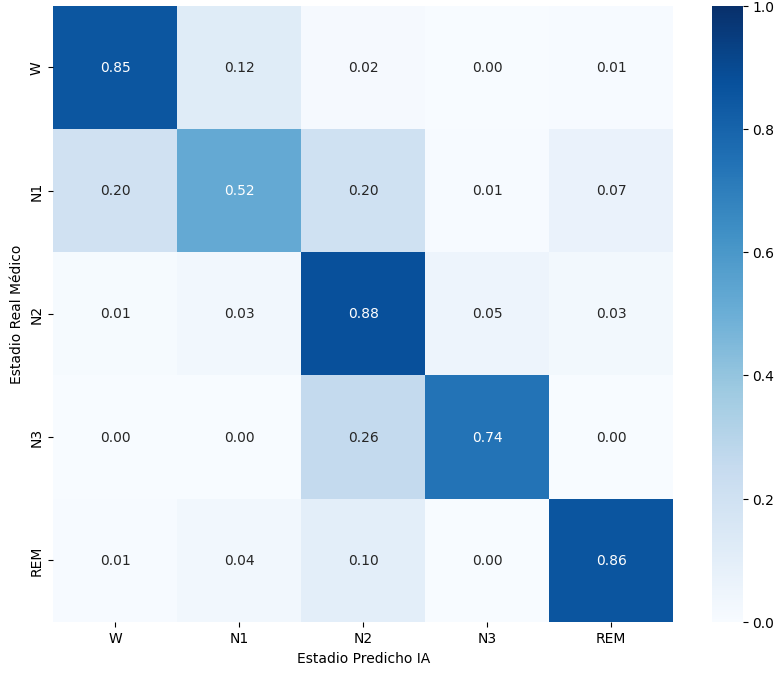
\includegraphics[width=\linewidth]{matriz_v4_interna.png}
        \caption{Validación Interna (V4)}
        \label{fig:matriz_a}
    \end{subfigure}\hfill
    % Panel B: Domain Shift V4 (Hold-Out limpio)
    \begin{subfigure}{0.32\textwidth}
        \centering
        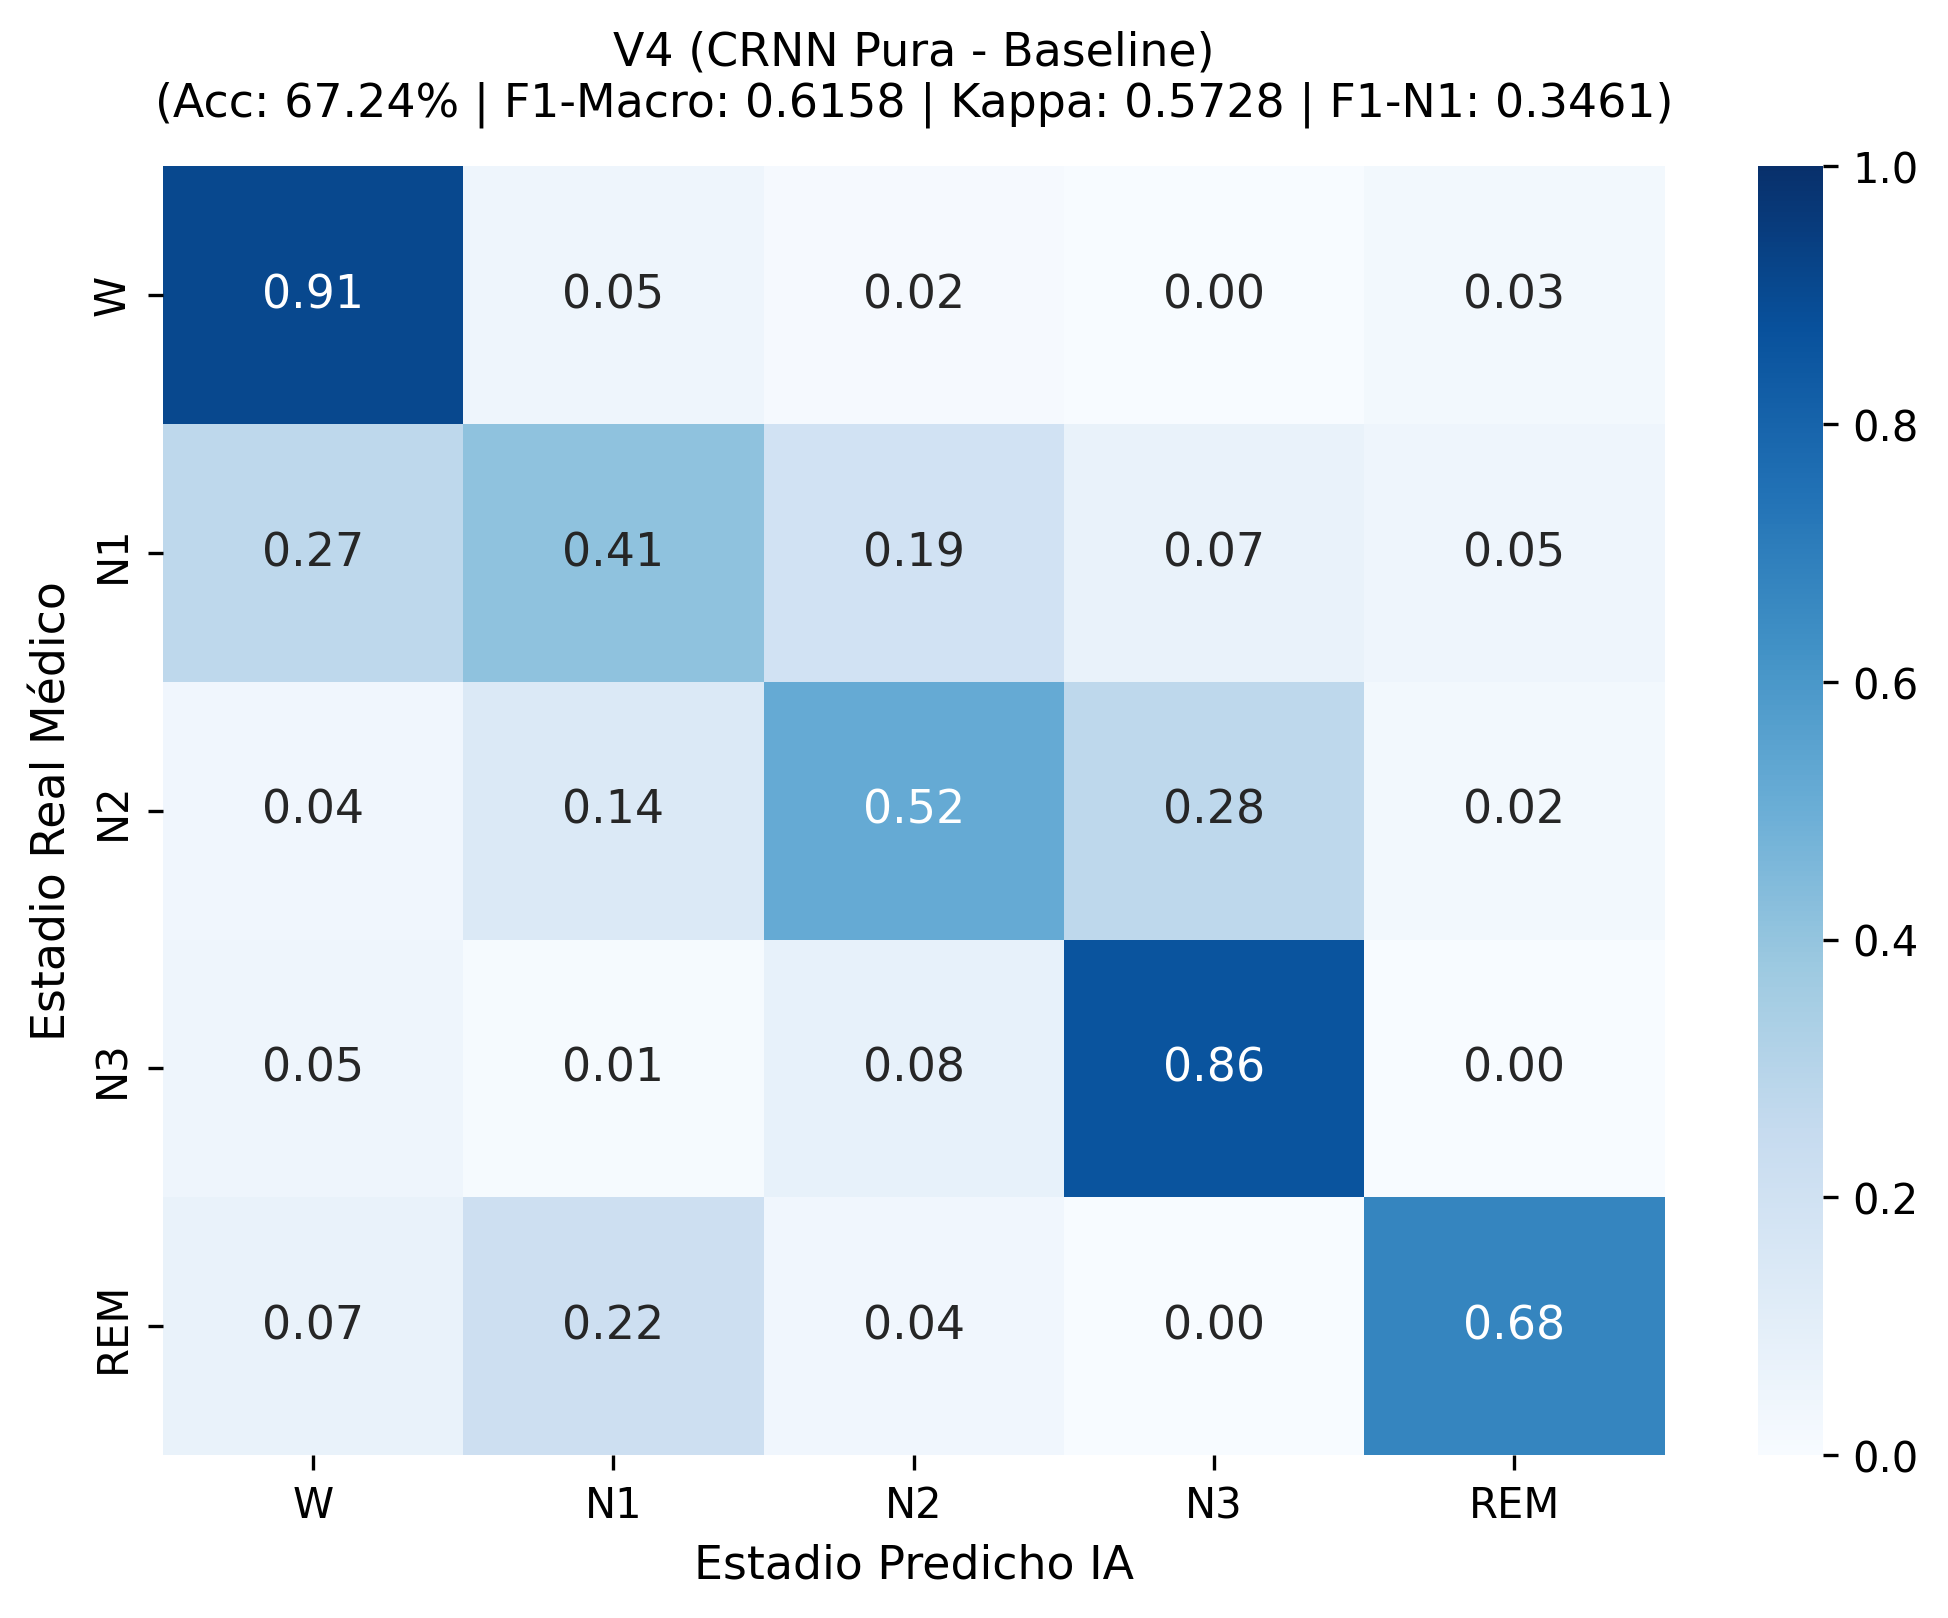
\includegraphics[width=\linewidth]{01_matriz_v4_crnn_pura_baseline.png}
        \caption{Domain Shift en Hold-Out (V4)}
        \label{fig:matriz_b}
    \end{subfigure}\hfill
    % Panel C: Recuperación V7 Exp 4 (Hold-Out limpio)
    \begin{subfigure}{0.32\textwidth}
        \centering
        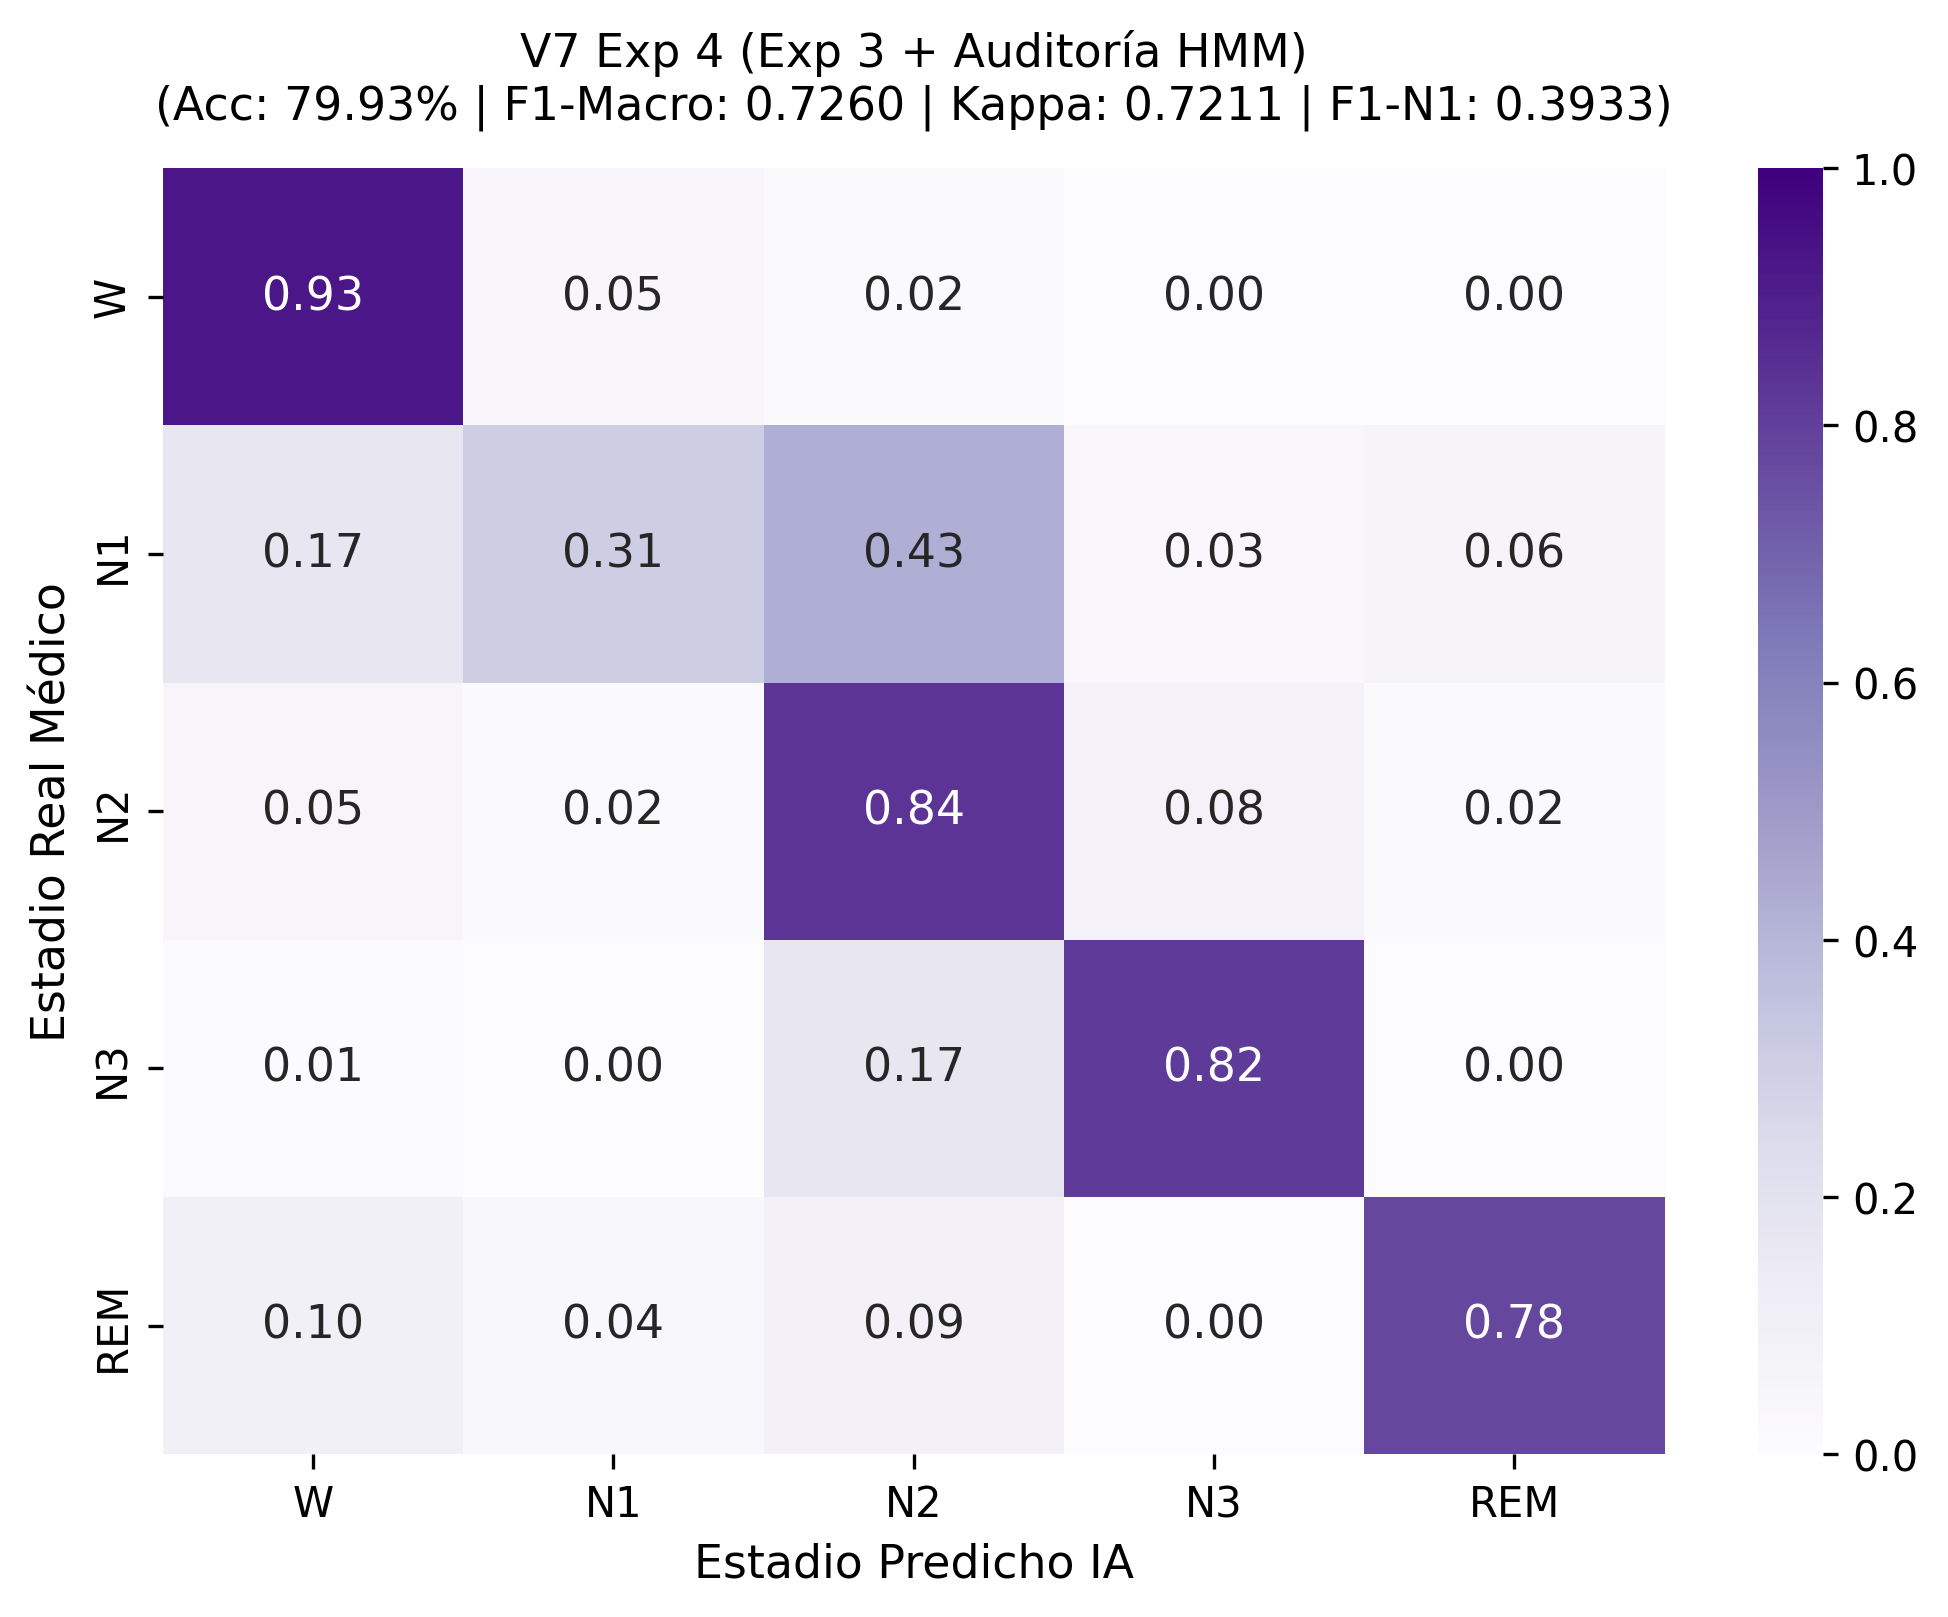
\includegraphics[width=\linewidth]{11_matriz_v7_exp_4.png}
        \caption{Recuperación (V7 Exp 4)}
        \label{fig:matriz_c}
    \end{subfigure}

\caption{Impacto visual del \textit{Domain Shift} y el entrenamiento multicohorte con fusión espectral. (a) La validación interna muestra una alta densidad en la diagonal principal. (b) La CRNN fundacional (V4) se degrada al enfrentarse a la cohorte externa. (c) La fusión espectral 528D y el filtro HMM (V7 Exp 4) restauran la estabilidad diagnóstica.}
\label{fig:matrices_confusion}
\end{figure*}

\subsection{Sensibilidad por Estadio y Análisis Visual}
El Cuadro \ref{tab:clinical_metrics} desglosa el F1-Score por clase AASM a lo largo de todas las fases evaluadas en el \textit{Hold-Out} limpio. Desde la línea base V4 hasta V7, los estadios consolidados mostraron recuperaciones claras: N2 pasó de 0.64 a 0.82, N3 de 0.48 a 0.70 y REM de 0.74 a 0.83. En N1, la rama espectral y los pesos de clase (Exp 1 a Exp 3) mantuvieron un F1 de 0.41, mientras que el HMM (Exp 4) mejoró REM (0.83) y el rendimiento global a costa de reducir F1-N1 a 0.39. Visualmente, la Figura \ref{fig:matrices_confusion}(c) confirma la recuperación de la diagonal principal en los estadios consolidados (W, N2, N3 y REM), concentrándose la confusión residual de N1 en su frontera fisiológica natural con N2 y W.

\begin{table}[htbp]
\centering
\caption{Comparativa de F1-Score por Estadio en Validación Externa Limpia}
\label{tab:clinical_metrics}
\resizebox{\columnwidth}{!}{%
\begin{tabular}{|l|c|c|c|c|c|}\textbf{}
\hline
\textbf{Versión del Sistema} & \textbf{W} & \textbf{N1} & \textbf{N2} & \textbf{N3} & \textbf{REM} \\ \hline
V4 (CRNN Pura - \textit{Baseline}) & 0.87 & 0.35 & 0.64 & 0.48 & 0.74 \\ \hline
V4 (Ensamble LightGBM Simple) & 0.85 & 0.38 & 0.70 & 0.51 & 0.77 \\ \hline
V4 (LGBM Telemetry+Cassette) & 0.87 & 0.39 & 0.78 & 0.60 & 0.77 \\ \hline
V5 Base (CRNN + \textit{Data Augmentation}) & 0.86 & 0.39 & 0.73 & 0.58 & \textbf{0.85} \\ \hline
V5 Base (LightGBM) & 0.86 & \textbf{0.41} & 0.78 & 0.66 & 0.83 \\ \hline
V5 Óptimo (CRNN + \textit{Data Augmentation}) & 0.86 & \textbf{0.41} & 0.75 & 0.61 & 0.82 \\ \hline
V5 Óptimo (LightGBM Optuna) & 0.87 & \textbf{0.41} & 0.80 & 0.67 & 0.81 \\ \hline
V6 Fase B (Contexto 192D) & \textbf{0.88} & \textbf{0.41} & 0.81 & 0.67 & 0.81 \\ \hline
V6 Fase C (Suavizado HMM) & 0.87 & 0.39 & 0.81 & 0.67 & 0.83 \\ \hline
V6 Fase D (TTA + HMM) & 0.87 & 0.38 & 0.81 & 0.68 & 0.83 \\ \hline
V7 Exp 1 (+ Bloques Espectrales 5s, 336D) & \textbf{0.88} & \textbf{0.41} & \textbf{0.82} & 0.69 & 0.82 \\ \hline
V7 Exp 2 (+ Norm. Nocturna P10--P90, 528D) & \textbf{0.88} & \textbf{0.41} & \textbf{0.82} & \textbf{0.70} & 0.82 \\ \hline
V7 Exp 3 (+ Pesos \texttt{Agresivo\_N1}, 528D) & \textbf{0.88} & \textbf{0.41} & \textbf{0.82} & \textbf{0.70} & 0.82 \\ \hline
\textbf{V7 Exp 4 (Exp 3 + Auditoría HMM)} & \textbf{0.88} & 0.39 & \textbf{0.82} & \textbf{0.70} & 0.83 \\ \hline
\end{tabular}%
}
\end{table}

\subsection{Contexto frente al Estado del Arte}
El Cuadro \ref{tab:sota_comparison} sitúa los resultados de V7 junto a referentes publicados sobre \textit{Sleep-EDF}. Dado que los protocolos no son directamente comparables (los trabajos previos reportan validación cruzada interna sobre particiones más extensas de \textit{Sleep-EDF}, mientras aquí se evalúa un conjunto fijo de 20 noches disjuntas por sujeto), las cifras propuestas se ubican ligeramente por debajo de dichas referencias, mostrando un desempeño razonable en estadios consolidados bajo un esquema híbrido modular.

\begin{table}[htbp]
\centering
\caption{Referencia Contextual frente al Estado del Arte en \textit{Sleep-EDF} (Protocolos No Equivalentes)}
\label{tab:sota_comparison}
\resizebox{\columnwidth}{!}{%
\begin{tabular}{|l|l|c|c|c|}
\hline
\textbf{Modelo / Estudio} & \textbf{Protocolo Reportado} & \textbf{Acc.} & \textbf{F1-M} & \textbf{Kappa} \\ \hline
DeepSleepNet \cite{supratak2017} & 20-Fold CV (Sleep-EDF-20) & 0.820 & 0.769 & 0.76 \\ \hline
TinySleepNet \cite{supratak2020} & 10-Fold CV (Sleep-EDF-78) & 0.831 & 0.781 & 0.77 \\ \hline
AttnSleep \cite{eldele2021} & 20-Fold CV (Sleep-EDF-78) & 0.813 & 0.751 & 0.74 \\ \hline
U-Sleep \cite{perslev2021} & CV Multi-cohorte (EDF-153) & --- & 0.790 & --- \\ \hline
\textbf{Propuesto (V7 Exp 3)} & \textbf{Val. Externa (20 noches)} & \textbf{0.797} & \textbf{0.729} & \textbf{0.72} \\ \hline
\textbf{Propuesto (V7 Exp 4)} & \textbf{Val. Externa (20 noches)} & \textbf{0.799} & \textbf{0.726} & \textbf{0.72} \\ \hline
\end{tabular}%
}
\end{table}

%===========================================================
\section{Discusión y Limitaciones}
%===========================================================
\textbf{Compromiso del HMM y Sensibilidad en N1:}
La Fase IV (V7) confirmó la hipótesis planteada: añadir bloques espectrales de 5 s y normalización nocturna ($P_{10}$--$P_{90}$) mejoró el equilibrio multiclase respecto a V6 (de 0.7139 a 0.7286 en \textit{F1-Macro} en Exp 3). Al aplicar HMM (Exp 4), se observó un compromiso claro: Viterbi eleva el \textit{Accuracy} al 79.93\%, el Kappa a 0.7211 y mejora REM (0.83), pero absorbe transiciones breves de N1 hacia N2 (F1-N1 baja de 0.41 a 0.39). Esto permite ofrecer dos perfiles configurables según la prioridad clínica.

\textbf{Normalización Nocturna y Resiliencia Arquitectónica:}
La normalización robusta por noche completa transforma la rama espectral a un enfoque retrospectivo (\textit{stateful}), compatible con la práctica clínica habitual donde el estudio se analiza tras el despertar. Asimismo, el diseño con \textit{Zero Imputation} permite ejecutar inferencia sin fallos de \textit{software} ante canales auxiliares faltantes (siempre que exista al menos un canal EEG), aunque su degradación cuantitativa deberá medirse empíricamente en trabajos futuros.

\textbf{Limitaciones del Estudio:}
Este trabajo presenta tres limitaciones metodológicas que deben considerarse al interpretar los resultados: (1) aunque el conjunto de 20 noches de \textit{Cassette} es estrictamente disjunto por sujeto respecto al entrenamiento, se reutilizó a lo largo de las fases V4--V7 para guiar decisiones de diseño, por lo que actuó como validación externa fija y no como prueba ciega evaluada una sola vez; (2) las diferencias pequeñas entre configuraciones (ej., Exp 2 vs. Exp 3) no cuentan con intervalos de confianza por \textit{bootstrap} a nivel de sujeto ni pruebas estadísticas pareadas; y (3) no se incluyeron ablaciones empíricas de desconexión de canales ni mediciones de latencia o validación clínica del flujo \textit{Human-in-the-Loop} en \textit{SleepAI Studio}.

%===========================================================
\section{Conclusiones y Trabajo Futuro}
%===========================================================
\subsection{Conclusiones}
El sistema híbrido propuesto (V7) demostró que acoplar una CRNN multimodal congelada (192D) con descriptores espectrales sub-época de 5 s, normalización nocturna ($P_{10}$--$P_{90}$) y contexto multiescala (528D) en LightGBM mejora consistentemente la clasificación frente a un esquema estrictamente local por época. Sobre el conjunto de validación externa fijo de 20 noches disjuntas por sujeto (10 sujetos de \textit{Sleep-Cassette}), el perfil Exp 3 alcanzó 79.71\% de \textit{Accuracy}, 0.7286 en \textit{F1-Macro}, 0.7188 en Kappa y 0.41 en F1-N1, mientras que el perfil con auditoría HMM (Exp 4) obtuvo 79.93\% de \textit{Accuracy}, 0.7260 en \textit{F1-Macro}, 0.7211 en Kappa y 0.39 en F1-N1, logrando un desempeño sólido en estadios consolidados (W, N2, N3 y REM).

\subsection{Trabajo Futuro}
Las siguientes etapas se centrarán en: (1) evaluar el modelo en cohortes externas completamente independientes con patologías severas (ej., SHHS y MESA del NSRR) incorporando intervalos de confianza por \textit{bootstrap}; (2) ejecutar pruebas empíricas de tolerancia a pérdida de canales, latencia de inferencia y calibración de incertidumbre para validar el flujo \textit{Human-in-the-Loop} en \textit{SleepAI Studio}; y (3) explorar los \textit{embeddings} latentes y el hipnograma como biomarcadores predictivos de patologías, en línea con los modelos fundacionales multimodales recientes \cite{thapa2026nature}.

%===========================================================
\section*{Declaraciones}
%===========================================================
\textbf{Disponibilidad de Datos y Ética:} Se utilizaron datos públicos y anonimizados de \textit{Sleep-EDF Database Expanded} alojados en PhysioNet bajo licencia abierta (ODC-By 1.0). \textbf{Conflicto de Intereses y Financiación:} Los autores declaran no tener conflictos de intereses; este trabajo fue desarrollado sin financiación externa en el marco de la Maestría en Inteligencia Artificial de la Universidad de los Andes. \textbf{Contribución de Autores:} Todos los autores contribuyeron equitativamente en la conceptualización, implementación, análisis de resultados y redacción del manuscrito.

\textbf{Uso de Inteligencia Artificial Generativa:} Durante la preparación de este trabajo, los autores utilizaron Google Gemini como herramienta de apoyo para la lluvia de ideas sobre refinamientos arquitectónicos, asistencia en la generación y depuración de código en Python, y revisión de estilo y redacción académica. Tras emplear esta herramienta, los autores revisaron, ejecutaron y validaron de forma independiente todo el código, los experimentos y el contenido del manuscrito, asumiendo plena responsabilidad por la integridad y exactitud de la publicación.

%===========================================================
\renewcommand{\refname}{Referencias}
\begin{thebibliography}{99}
%===========================================================

\bibitem{berry2020}
R. B. Berry, R. Brooks, C. E. Gamaldo, S. M. Harding, R. M. Lloyd, C. L. Marcus, y B. V. Vaughn, \textit{The AASM Manual for the Scoring of Sleep and Associated Events: Rules, Terminology and Technical Specifications}. Darien, IL, EE. UU.: American Academy of Sleep Medicine, 2020.

\bibitem{kemp2000}
B. Kemp \textit{et al.}, ``Analysis of a sleep-dependent neuronal feedback loop: the slow-wave microcontinuity of the EEG,'' \textit{IEEE Transactions on Biomedical Engineering}, vol. 47, no. 9, pp. 1185--1194, 2000, doi: \url{https://doi.org/10.1109/10.867928}.

\bibitem{supratak2020}
A. Supratak y Y. Guo, ``TinySleepNet: An efficient deep learning model for sleep stage scoring based on raw single-channel EEG,'' en \textit{Proc. 42nd Annu. Int. Conf. IEEE Eng. Med. Biol. Soc. (EMBC)}, 2020, pp. 641--644, doi: \url{https://doi.org/10.1109/EMBC44109.2020.9176741}.

\bibitem{ke2017}
G. Ke \textit{et al.}, ``LightGBM: A highly efficient gradient boosting decision tree,'' en \textit{Advances in Neural Information Processing Systems (NeurIPS)}, vol. 30, 2017.

\bibitem{supratak2017}
A. Supratak, H. Dong, C. Wu, y Y. Guo, ``DeepSleepNet: A model for automatic sleep stage scoring based on raw single-channel EEG,'' \textit{IEEE Transactions on Neural Systems and Rehabilitation Engineering}, vol. 25, no. 11, pp. 1998--2008, 2017, doi: \url{https://doi.org/10.1109/TNSRE.2017.2721116}.

\bibitem{perslev2021}
M. Perslev, S. Darkner, L. Kempfner, M. Nikolic, P. J. Jennum, y C. Igel, ``U-Sleep: resilient high-frequency sleep staging,'' \textit{npj Digital Medicine}, vol. 4, no. 1, art. 72, 2021, doi: \url{https://doi.org/10.1038/s41746-021-00440-5}.

\bibitem{phan2023}
H. Phan \textit{et al.}, ``L-SeqSleepNet: Whole-cycle long sequence modeling for automatic sleep staging,'' \textit{IEEE Journal of Biomedical and Health Informatics}, vol. 27, no. 10, pp. 4748--4757, 2023, doi: \url{https://doi.org/10.1109/JBHI.2023.3303197}.

\bibitem{eldele2021}
E. Eldele \textit{et al.}, ``An attention-based deep learning approach for sleep stage classification with single-channel EEG,'' \textit{IEEE Transactions on Neural Systems and Rehabilitation Engineering}, vol. 29, pp. 809--818, 2021, doi: \url{https://doi.org/10.1109/TNSRE.2021.3076234}.

\bibitem{geirhos2020shortcut}
R. Geirhos, J.-H. Jacobsen, C. Michaelis, R. Zemel, W. Brendel, M. Bethge, y F. A. Wichmann, ``Shortcut learning in deep neural networks,'' \textit{Nature Machine Intelligence}, vol. 2, no. 11, pp. 665--673, 2020, doi: \url{https://doi.org/10.1038/s42256-020-00257-z}.

\bibitem{sleepedfx_dataset}
B. Kemp, A. H. Zwinderman, B. Tuk, H. A. Kamphuisen, y J. J. Oberyé, ``Sleep-EDF Database Expanded (version 1.0.0),'' \textit{PhysioNet}, 2018, doi: \url{https://doi.org/10.13026/C2X676}.

\bibitem{goldberger2000}
A. L. Goldberger \textit{et al.}, ``PhysioBank, PhysioToolkit, and PhysioNet: components of a new research resource for complex physiologic signals,'' \textit{Circulation}, vol. 101, no. 23, pp. e215--e220, 2000, doi: \url{https://doi.org/10.1161/01.cir.101.23.e215}.

\bibitem{gramfort2013}
A. Gramfort \textit{et al.}, ``MEG and EEG data analysis with MNE-Python,'' \textit{Frontiers in Neuroscience}, vol. 7, art. 267, 2013, doi: \url{https://doi.org/10.3389/fnins.2013.00267}.

\bibitem{akiba2019optuna}
T. Akiba, S. Sano, T. Yanase, T. Ohta, y M. Koyama, ``Optuna: A next-generation hyperparameter optimization framework,'' en \textit{Proc. 25th ACM SIGKDD Int. Conf. Knowl. Discov. Data Min.}, 2019, pp. 2623--2631, doi: \url{https://doi.org/10.1145/3292500.3330701}.

\bibitem{lin2017}
T.-Y. Lin, P. Goyal, R. Girshick, K. He, y P. Dollár, ``Focal loss for dense object detection,'' en \textit{Proc. IEEE Int. Conf. Comput. Vis. (ICCV)}, 2017, pp. 2980--2988, doi: \url{https://doi.org/10.1109/ICCV.2017.324}.

\bibitem{thapa2026nature}
R. Thapa \textit{et al.}, ``A multimodal sleep foundation model for disease prediction,'' \textit{Nature Medicine}, vol. 32, pp. 752--762, 2026, doi: \url{https://doi.org/10.1038/s41591-025-04133-4}.

\end{thebibliography}

\end{document}